%%%%%%%%%%%%%%%%%%%%%%%%%%%%%%%%%%%%%%%%%%%%%%%%%%%%%%%%%%%%%%%%%%%%%%%%%%%%%%%%%%%%%%%%%%%%%%%%%%%%%
% This template is distributed with ABSOLUTELY NO WARRANTY.
% It serves as a guideline and constitutes a basic structure for a
% thesis/dissertation. The user assumes full responsibility for formatting
% and typesetting their document and for verifying that all the thesis
% requirements set by the University of Tennessee are met. Please refer to the most
% recent UT thesis guide (http://web.utk.edu/~thesis/thesisresources.shtml)
% or contact the thesis consultant (http://web.utk.edu/~thesis/).
% Please report any bugs to the thesis consultant.
%%%%%%%%%%%%%%%%%%%%%%%%%%%%%%%%%%%%%%%%%%%%%%%%%%%%%%%%%%%%%%%%%%%%%%%%%%%%%%%%%%%%%%%%%%%%%%%%%%%%%
% O P T I O N S:
% 1. thesis/dissertation
% 2. monochrome
% 3. all options provided by the report class
\documentclass[thesis,letterpaper,12pt]{utthesis} % thesis, one side
% some alternatives are:
%\documentclass[thesis,monochrome,letterpaper,12pt]{utthesis} %thesis, one side, monochrome text
%\documentclass[thesis,twoside,letterpaper,12pt]{utthesis} % thesis, two side
%\documentclass[thesis,monochrome,twoside,letterpaper,12pt]{utthesis} % thesis, two side, monochrome text
% for a dissertation, replace the thesis option by dissertation:
% \documentclass[dissertation,letterpaper,12pt]{utthesis} . . .
\renewcommand{\baselinestretch}{1.5} 	 % line Spacing
%%%%%%%%%%%%%%%%%%%%%%%%%%%%%%%%%%%%%%%%%%%%%%%%%%%%%%%%%%%%%%%%%%%%%%%%%%%%%%%%%%%%%%%%%%%%%%%%%%%%%
% TO DO: FILL IN YOUR INFORMATION BELOW - READ THIS SECTION CAREFULLY
%%%%%%%%%%%%%%%%%%%%%%%%%%%%%%%%%%%%%%%%%%%%%%%%%%%%%%%%%%%%%%%%%%%%%%%%%%%%%%%%%%%%%%%%%%%%%%%%%%%%%
\title{Correction to Luminosity Measurement for the Pixel Luminosity Telescope at CMS}	       % title of thesis/dissertation
\author{Krishna Thapa}                % author's name
\copyrightYear{2016}            % copyright year of your thesis/dissertation
\graduationMonth{December}           % month of graduation of your thesis/dissertation
\majorProfessor{Stefan M. Spanier}	    % advisor's name
\keywords{List, Of, Keywords}	% keywords (optional) separated by commas - these are used in the PDF file properties
\viceProvost{Carolyn R. Hodges} % vice provost name
\major{High Energy Physics}	% major: Mechanical Engineering, Aerospace Engineering, Mathematics...
\degree{Master of Science}	    % degree: Doctor of Philosophy, Master of Science, Master of Engineering...
\college{Engineering}           % college
\dept{Mechanical, Aerospace and Biomedical Engineering}	% department
\university{The University  of Tennessee, Knoxville}	% school name
% THIS TEMPLATE ACCOMMODATES UP TO 5 COMMITTEE MEMBERS - ENTER ONLY THE NAMES OF THE MEMBERS ON YOUR COMMITTEE
\numberOfCommitteeMembers{3} % enter the number of committee members
\committeeMemberA {Dr. Stefan Spanier}	% name of first committee member
\committeeMemberB {Dr. Marinne Breining}	% name of second committee member
\committeeMemberC {Dr. Thomas Handler}	% ... you get the trend!
\committeeMemberD {Committee Member 4}	% if your committee has less than 4 members, you do not need to edit the
\committeeMemberE {Committee Member 5}  % rest of committee names
%%%%%%%%%%%%%%%%%%%%%%%%%%%%%%%%%%%%%%%%%%%%%%%%%%%%%%%%%%%%%%%%%%%%%%%%%%%%%%%%%%%%%%%%%%%%%%%%%%%%%
% LOAD SOME USEFUL PACKAGES
%%%%%%%%%%%%%%%%%%%%%%%%%%%%%%%%%%%%%%%%%%%%%%%%%%%%%%%%%%%%%%%%%%%%%%%%%%%%%%%%%%%%%%%%%%%%%%%%%%%%%
\usepackage{nomencl}                    % produces a nomenclature
\usepackage{float}                      % figure floats
\usepackage{natbib}                     % this package allows you to link your references
\usepackage{graphicx}					% graphics package
\graphicspath{ {figures/}{figures/eps/}{figures/pdf/} }% specify the path where figures are located
\usepackage{fancyhdr}                   % fancy headers and footers
\usepackage{url}                        % nicely format url breaks
\usepackage[inactive]{srcltx}		 	% necessary to use forward and inverse searching in DVI
\usepackage{relsize}                    % font sizing hierarchy
\usepackage{booktabs}                   % professional looking tables
\usepackage[config, labelfont={bf}]{caption,subfig} % nice sub figures
\usepackage{mathrsfs}                   % additional math scripts


% does not recognize png extension, sometimes
%\usepackage{graphicx}
\usepackage{grffile}
%\usepackage{subcaption}
%\usepackage{floatrow}
%\usepackage{pst-plot}

% for tikz
\usepackage{pgfplots}

\usepgfplotslibrary{polar}
\usepgflibrary{shapes.geometric}
\usetikzlibrary{calc}


\usepackage{tikz}
\usepackage{tkz-euclide}
\usetkzobj{all}
\usetikzlibrary{decorations.text,calc,arrows.meta}

% convert ps to pdf
%\usepackage{auto-pst-pdf}

% to indent caption
% http://tex.stackexchange.com/questions/149752/indent-figure-multi-line-caption
\usepackage{caption}

%code environement
\usepackage{listings}
\usepackage{xcolor}
%\lstset{escapechar=@,style=customc}

%http://tex.stackexchange.com/questions/81834/whats-the-best-way-to-typeset-c-codes-in-latex
\definecolor{listinggray}{gray}{0.9}
\definecolor{lbcolor}{rgb}{0.9,0.9,0.9}
\lstset{
backgroundcolor=\color{lbcolor},
    tabsize=4,    
%   rulecolor=,
    language=[GNU]C++,
        basicstyle=\scriptsize,
        upquote=true,
        aboveskip={1.5\baselineskip},
        columns=fixed,
        showstringspaces=false,
        extendedchars=false,
        breaklines=true,
        prebreak = \raisebox{0ex}[0ex][0ex]{\ensuremath{\hookleftarrow}},
        frame=single,
%        numbers=left,
        showtabs=false,
        showspaces=false,
        showstringspaces=false,
        identifierstyle=\ttfamily,
        keywordstyle=\color[rgb]{0,0,1},
        commentstyle=\color[rgb]{0.026,0.112,0.095},
        stringstyle=\color[rgb]{0.627,0.126,0.941},
%        numberstyle=\color[rgb]{0.205, 0.142, 0.73},
%        \lstdefinestyle{C++}{language=C++,style=numbers}?.
}
\lstset{
  backgroundcolor=\color{lbcolor},
   tabsize=4,
  language=C++,
  captionpos=b,
  tabsize=3,
  frame=lines,
%  numbers=left,
%  numberstyle=\tiny,
%  numbersep=5pt,
  breaklines=true,
  showstringspaces=false,
  basicstyle=\footnotesize,
%  identifierstyle=\color{magenta},
  keywordstyle=\color[rgb]{0,0,1},
  commentstyle=\color{Darkgreen},
  stringstyle=\color{red}
  }
  
  \lstdefinestyle{customc}{
  belowcaptionskip=1\baselineskip,
  breaklines=true,
  frame=L,
  xleftmargin=\parindent,
  language=C,
  showstringspaces=false,
  basicstyle=\footnotesize\ttfamily,
  keywordstyle=\bfseries\color{green!40!black},
  commentstyle=\itshape\color{purple!40!black},
  identifierstyle=\color{blue},
  stringstyle=\color{orange},
}
\lstset{escapechar=@,style=customc}  


%%% PACKAGES THAT ARE PRELOADED WITH THE CLASS ARE: amsmath,amsthm,amssymb,setspace,geometry,hyperref,and color
%%%%%%%%%%%%%%%%%%%%%%%%%%%%%%%%%%%%%%%%%%%%%%%%%%%%%%%%%%%%%%%%%%%%%%%%%%%%%%%%%%%%%%%%%%%%%%%%%%%%%
\begin{document}
    \pagenumbering{alph} % this is needed to clear certain issues with the hyperref package
    %
    \makeApprovalPage % make the approval page - this is the page that needs to be signed & returned to the thesis/dissertation consultant
    \makeETDApprovalPage % make the Electronic Thesis & Dissertation page - this page is kept with the electronic copy
    %
    \addToPDFBookmarks{0}{Front Matter}{rootNode} % create a root node named "Front Matter" in the pdf bookmarks
    \addToPDFBookmarks{1}{Title}{a} % add a pdf bookmark to the title page
    \makeTitlePage % make the title page. Make sure you properly set the \docType
    %
    \pagenumbering{roman}
    \setcounter{page}{2}
    %
    \makeCopyrightPage % make the copyright page
    %
    \addToPDFBookmarks{1}{Dedication}{b} % add a pdf bookmark to the dedication page
    \chapter*{}
\begin{center}
{\centering \it dedication... }
\end{center}  % include the dedication
    %
    \addToPDFBookmarks{1}{Acknowledgements}{c} % add a pdf bookmark to the acknowledgements page
    \chapter*{Acknowledgements}
I would like to thank... % include the acknowledgements
    %
    \addToPDFBookmarks{1}{Quote}{d} % add a pdf bookmark to the quotation page
    \chapter*{}
{\it Some quotation...} % include a quote
    %
    \addToPDFBookmarks{1}{Abstract}{e} % add a pdf bookmark to the abstract page
    \chapter*{Abstract}\label{ch:abstract}
Abstract text goes here... % your abstract
    %
    \addToPDFBookmarks{0}{Table of Contents}{f}
    \tableofcontents % generate a table of contents
    %
    \addToTOC{List of Tables} % this will add the list of tables to the Table of Contents (TOC)
    \listoftables % generate a list of tables
    %
    \addToTOC{List of Figures} % this will add the list of figures to the Table of Contents (TOC)
    \listoffigures % generate a list of figures
    %
    \makenomenclature % OPTIONAL
    \addToPDFBookmarks{0}{Nomenclature}{g} % OPTIONAL
    \printnomenclature[1.25in] % OPTIONAL
    %
    \newpage
    \pagenumbering{arabic}
    \setcounter{page}{1}
    %%%%%%%%%%%%%%%%%%%%%%%%%%%%%%%%%%%%%%%%%%%%%%%%%%%%%%%%%%%%%%%%%%%%%%%%%%%%%%%%%%%%%%%%%%%%%%%%%%%%%
    % INCLUDE THE CHAPTERS STARTING WITH THE NOMENCLATURE IF PRESENT
    %%%%%%%%%%%%%%%%%%%%%%%%%%%%%%%%%%%%%%%%%%%%%%%%%%%%%%%%%%%%%%%%%%%%%%%%%%%%%%%%%%%%%%%%%%%%%%%%%%%%%
    % enter the list of nomenclature here
\nomenclature{$r$}{Radial coordinate}
\nomenclature{$\theta$}{Tangential coordinate}
\nomenclature{$z$}{Axial coordinate}
\nomenclature{$\bar{}$}{Denotes a dimensional variable}
\nomenclature{$\psi$}{Streamfunction}
\nomenclature{$u_r$}{Radial velocity}%
\nomenclature{$u_{\theta}$}{Tangential velocity}%
\nomenclature{$u_z$}{Axial velocity}%
\nomenclature{$p$}{Pressure} 
 % OPTIONAL
    \chapter{Introduction} \label{ch:introduction}

This is a very short guide to an unofficial thesis/dissertation template for the University of Tennessee. It is based on the 2010 thesis specifications but can be easily altered as the guidelines are changed. This template requires a basic knowledge of \LaTeX\ and should cover the basic requirements in terms of required packages and functionality.

\section{Disclaimer}
\textcolor{red}{\bf
This template is distributed with ABSOLUTELY NO WARRANTY. It serves as a guideline and constitutes a basic structure for a thesis/dissertation. The user assumes full responsibility for formatting and typesetting their document and for verifying that all the thesis requirements set by the University of Tennessee are met. Please refer to the most recent UT thesis guide \href{http://web.utk.edu/~thesis/thesisresources.shtml}{http://web.utk.edu/~thesis/thesisresources.shtml} or contact the thesis consultant (\href{http://web.utk.edu/~thesis/}{http://web.utk.edu/~thesis/}). Please report any bugs to the thesis consultant.}

\section{Getting started}
\begin{figure}[b!]
  \centering
  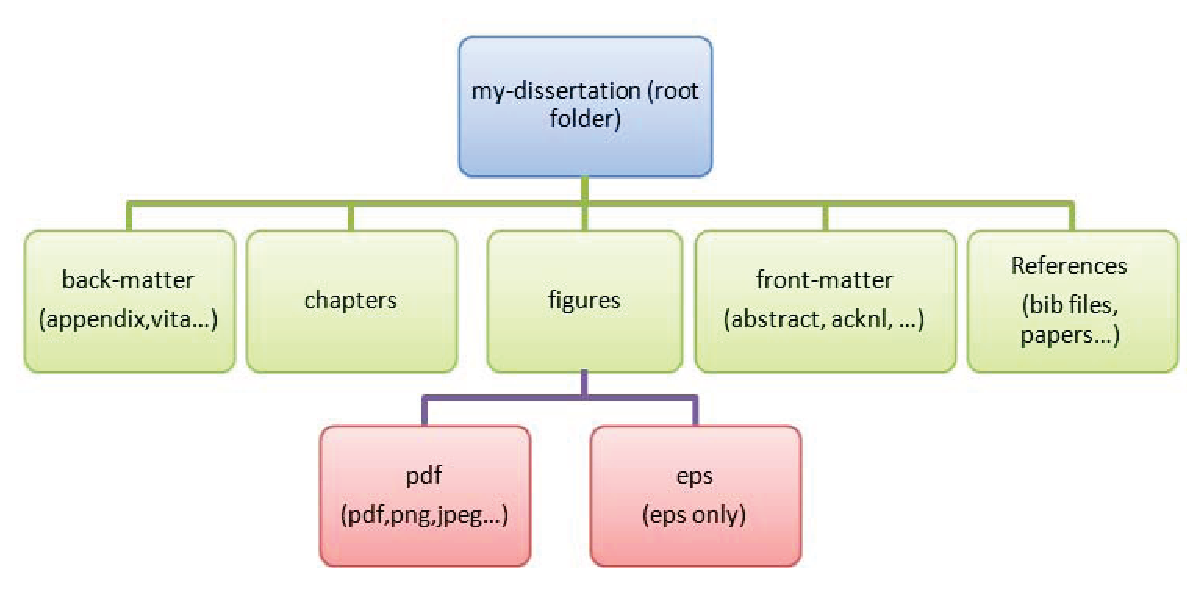
\includegraphics[width=6.5in]{fig01-folder-structure}\\
  \caption{UT thesis template folder structure.}\label{fig:intro-folder-structure}
\end{figure}
The general structure of this template is based on the tree shown in Figure \ref{fig:intro-folder-structure}. The titles of the folders are self descriptive and should guide you to proper file placement. Note that this is only a suggested model that could be modified to fit your own organizational structure.

There are two important files in this template: ``ut-thesis-template.tex'' and ``utthesis.cls''. The ``utthesis.cls'' is the class file that contains the settings, definitions, packages, and macros for this template to work properly and is located in the root directory. This file constitutes the document class for the template. It is based on the report class and provides some customized functionality. For example, it can automatically generate the signature pages for committees of up to five members. It will also generate a title page for you. In certain cases, one of the packages included in this template may conflict with a package that you are adding. You will have to resolve this conflict by either removing the package that is not being used or by modifying some settings with either packages. The packages that are preloaded in this class file are: amsmath, amsthm, amssymb, setspace, geometry, hyperref, and color.

The ``my-dissertation.tex'' file is the main file for your thesis/dissertation. This is where you should start editing and planning for your thesis/dissertation. You may want to change the name of the file to something like ``my-name-dissertation.tex''. Next, invoke the proper options for the ``utthesis'' document class. This class will take all the options for the report class in addition to two options: thesis/dissertation and monochrome. If you are writing a thesis, you must use "thesis" otherwise, use "dissertation" or omit that option because dissertation is the default setting. The monochrome option converts all your document to monochrome - except figures. This is very useful when printing your document. Because this dissertation has colored hyperlinks, these will look washed out when printed on a monochrome printer. Therefore, it is handy to have a monochrome copy of you3r thesis for print. Below are some examples of typical settings.
\begin{verbatim}
%%%%%%%%%%%%%%%%%%%%%%%%%%%%%%%%%%%%%%%%%%%%%%%%%%%%%%%%%%%%%%%%%%%%%%%%%%%
Thesis, color, one side
\documentclass[thesis,monochrome,letterpaper,12pt]{utthesis}
Thesis, monochrome, one side
\documentclass[thesis,monochrome,letterpaper,12pt]{utthesis}
Thesis, color, twoside side (good for binding)
\documentclass[thesis,twoside,letterpaper,12pt]{utthesis}
Thesis, monochrome, twoside side (good for binding)
\documentclass[thesis,monochrome,twoside,letterpaper,12pt]{utthesis}
Dissertation, color, one side
\documentclass[dissertation,letterpaper,12pt]{utthesis}
Dissertation, monochrome, two side
\documentclass[dissertation,twoside,letterpaper,12pt]{utthesis} . . .
%%%%%%%%%%%%%%%%%%%%%%%%%%%%%%%%%%%%%%%%%%%%%%%%%%%%%%%%%%%%%%%%%%%%%%%%%%%
\end{verbatim}

Now you are ready to fill in the proper values corresponding to your name, degree, advisor etc... This can be done in the following section:
\begin{verbatim}
%%%%%%%%%%%%%%%%%%%%%%%%%%%%%%%%%%%%%%%%%%%%%%%%%%%%%%%%%%%%%%%%%%%%%%%%%%%
% TO DO: FILL IN YOUR INFORMATION BELOW - READ THIS SECTION CAREFULLY
%%%%%%%%%%%%%%%%%%%%%%%%%%%%%%%%%%%%%%%%%%%%%%%%%%%%%%%%%%%%%%%%%%%%%%%%%%%
\title{My Thesis or Dissertation Title}
\author{My Name}
\copyrightYear{2012}
\graduationMonth{May}
\majorProfessor{My Advisor}
\keywords{List, Of, Keywords}
\viceProvost{Carolyn R. Hodges}
\major{Mechanical Engineering}
\degree{Master of Science}
\college{Engineering}
\dept{Mechanical, Aerospace and Biomedical Engineering}
\university{The University  of Tennessee, Knoxville}
\numberOfCommitteeMembers{2}
\committeeMemberA {Committee Member 1}
\committeeMemberB {Committee Member 2}
\committeeMemberC {Committee Member 3}
\committeeMemberD {Committee Member 4}
\committeeMemberE {Committee Member 5}
%%%%%%%%%%%%%%%%%%%%%%%%%%%%%%%%%%%%%%%%%%%%%%%%%%%%%%%%%%%%%%%%%%%%%%%%%%%
\end{verbatim}
Note, that if you have less than five committee members, you will only need to fill in the names of your committee. The template will take care of the rest given that you provide the correct number of committee members. For example, if you have three members on your committee, you only need to fill in
\begin{verbatim}
\numberOfCommitteeMembers{3}
\committeeMemberA {Committee Member 1}
\committeeMemberB {Committee Member 2}
\committeeMemberC {Committee Member 3}
\end{verbatim}

\section{References}
The bibliography style used in this template is "apalike". It is an author-year style based on the APA specification. Here are a few examples. \cite{Fermi1956} wrote a book on thermodynamics. The book by \cite{liepmann2001} on gas dynamics is a classic textbook used in most courses on compressible flows. You can also use the citations at the end of a line \citep{Saad2010RSPA,Lamb1895}. For more information, visit \href{http://merkel.zoneo.net/Latex/natbib.php}{http://merkel.zoneo.net/Latex/natbib.php}.

\section{Theorem environments}
This template contains predefined theorem, lemma, and corollary environments. For example
\begin{theorem}[First theorem]\label{thm:theorem-a}
    This is an example theorem.
\end{theorem}
\begin{proof}[Proof for theorem] \ref{thm:theorem-a}
    This is the proof for this theorem.
\end{proof}
\begin{lemma}[First lemma]
    This is the first lemma.
\end{lemma}
\begin{corollary}
    This is the first corollary.
\end{corollary}

\newpage
\section{Figures}
\subsection{Single figures}
For more information, check: \href{http://en.wikibooks.org/wiki/LaTeX/Floats,_Figures_and_Captions}{http://en.wikibooks.org/wiki/LaTeX/Floats,\_Figures\_and\_Captions}
\begin{verbatim}
    \begin{figure}[t for top, b for bottom, h for here, ! to force placement]
        % Requires \usepackage{graphicx}
        \centering % center the figure
        \includegraphics[width=5in or 127mm etc...]{figure-name}\\
        \caption{figure caption}\label{figure label}
    \end{figure}
\end{verbatim}
\begin{figure}[h!]
  % Requires \usepackage{graphicx}
  \centering
  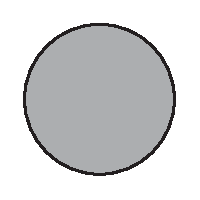
\includegraphics[width=3in]{fig02a-circle}\\
  \caption{Sample caption.}\label{label}
\end{figure}
\newpage
\subsection{Multipart figures}
For multipart figures, you need to use the package "subfig". here's an example
\begin{verbatim}
\begin{figure}
    \centering
    \subfloat[figure a]{\label{fig:figure-a} \includegraphics[width=w]{fig02a}}
    \subfloat[figure b]{\label{fig:figure-b} \includegraphics[width=w]{fig02b}}
    \subfloat[figure c]{\label{fig:figure-c} \includegraphics[width=w]{fig02c}}
    \caption{Sample of a multipart figure} \label{fig:multipart-figure}
\end{figure}
\end{verbatim}
\begin{figure}[h!]
        \centering
        \subfloat[Circle]{\label{fig:figure-a}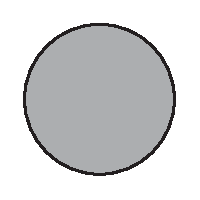
\includegraphics[width=1.1in]{fig02a-circle}}
        \subfloat[Rectangle]{\label{fig:figure-b}
\includegraphics[width=1.1in]{fig02b-rectangle}}
        \subfloat[Cube]{\label{fig:figure-c}
\includegraphics[width=1.1in]{fig02c-cube}}
        \caption{Geometric shapes.}
        \label{fig:multipart-figure}
\end{figure}
To add some space between the figures above, one can use the usual spacing commands such as ``qquad''
\begin{figure}[h!]
        \centering
        \subfloat[Circle]{\label{fig:figure-a}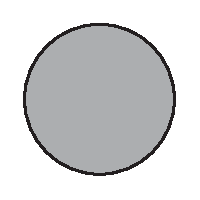
\includegraphics[width=1.1in]{fig02a-circle}} \qquad
        \subfloat[Rectangle]{\label{fig:figure-b}
\includegraphics[width=1.1in]{fig02b-rectangle}}\qquad
        \subfloat[Cube]{\label{fig:figure-c}
\includegraphics[width=1.1in]{fig02c-cube}}\qquad
        \caption{Geometric shapes.}
        \label{fig:multipart-figure}
\end{figure} 
    \chapter{Physics Background} \label{ch:physBKGD}

    \chapter{Experimental Setup} \label{ch:expSetup}
    
    \chapter{Conclusions} \label{ch:conclusion}
    \chapter{Conclusions} \label{ch:conclusion}
    \chapter{Conclusions} \label{ch:conclusion}
    
    %%%%%%%%%%%%%%%%%%%%%%%%%%%%%%%%%%%%%%%%%%%%%%%%%%%%%%%%%%%%%%%%%%%%%%%%%%%%%%%%%%%%%%%%%%%%%%%%%%%%%
    % BIBLIOGRAPHY
    %%%%%%%%%%%%%%%%%%%%%%%%%%%%%%%%%%%%%%%%%%%%%%%%%%%%%%%%%%%%%%%%%%%%%%%%%%%%%%%%%%%%%%%%%%%%%%%%%%%%%
    \makeBibliographyPage % make the bibliography title page - can be edited in ut-thesis-template.tex
    \bibliographystyle{apalike} % bibliography style - recommend using apalike-doi as it hyperlinks DOIs
    \bibliography{references/references-dissertation} % references.bib included in the references directory
    %%%%%%%%%%%%%%%%%%%%%%%%%%%%%%%%%%%%%%%%%%%%%%%%%%%%%%%%%%%%%%%%%%%%%%%%%%%%%%%%%%%%%%%%%%%%%%%%%%%%%
    % APPENDIX - OPTIONAL - COMMENT IF NOT NEEDED
    %%%%%%%%%%%%%%%%%%%%%%%%%%%%%%%%%%%%%%%%%%%%%%%%%%%%%%%%%%%%%%%%%%%%%%%%%%%%%%%%%%%%%%%%%%%%%%%%%%%%%
    \makeAppendixPage   % make the appendix title page - can be edited in ut-thesis-template.tex
    \appendix
    \chapter{Summary of Equations}
\section{Cartesian}
some equations here

\section{Cylindrical}
some equations also here
    %%%%%%%%%%%%%%%%%%%%%%%%%%%%%%%%%%%%%%%%%%%%%%%%%%%%%%%%%%%%%%%%%%%%%%%%%%%%%%%%%%%%%%%%%%%%%%%%%%%%%
    % A VITA IS REQUIRED
    %%%%%%%%%%%%%%%%%%%%%%%%%%%%%%%%%%%%%%%%%%%%%%%%%%%%%%%%%%%%%%%%%%%%%%%%%%%%%%%%%%%%%%%%%%%%%%%%%%%%%
    \addToTOC{Vita}
    \chapter*{Vita} \label{ch:vita}
Vita goes here...
\end{document}
